\documentclass[10pt,twocolumn]{article}

% Packages for layout and formatting
\usepackage[top=1in,bottom=1in,left=0.75in,right=0.75in]{geometry}
\usepackage{times}
\usepackage{graphicx}
\usepackage{multicol}
\usepackage{hyperref}
\usepackage{titlesec}
\usepackage{enumitem}
\usepackage{abstract}

% Reduce space between columns
\setlength{\columnsep}{0.25in}

% Section styling
\titleformat{\section}{\large\bfseries}{\thesection}{1em}{}
\titleformat{\subsection}{\normalsize\bfseries}{\thesubsection}{1em}{}

% Title setup
\title{\vspace{-1.5em}\textbf{CodeCurrent : Multi-language Functional Flow Visualization for Codebases}\\
\vspace{0.5em}}
\author{
  \begin{tabular}{ccc}
    Veerain Sood & Preet Bobde & Kowshik Reddy Challa\\
    \texttt{cs22b049@iittp.ac.in} & \texttt{cs22b043@iittp.ac.in} & \texttt{cs22b015@iittp.ac.in} \\
    \texttt{IIT Tirupati} & \texttt{IIT Tirupati} & \texttt{IIT Tirupati} \\ \\
    Anuj Sharma & Ashish Raj & Lavkush Kumar \\
    \texttt{cs22b007@iittp.ac.in} & \texttt{cs22b055@iittp.ac.in} & \texttt{cs22b034@iittp.ac.in}\\
    \texttt{IIT Tirupati} & \texttt{IIT Tirupati} & \texttt{IIT Tirupati} \\ \\
  \end{tabular} \\[1em]
  \textbf{Guided by: Dr. Sridhar Chimalakonda, IIT Tirupati}
}
\date{}



\begin{document}

\twocolumn[\maketitle]

% Abstract section
\noindent\textbf{Abstract:} 
Large-scale software systems often incorporate multiple programming languages such as Python, Java, and C++, posing significant challenges for developers attempting to understand the functional flow across the entire codebase. Navigating cross-language function calls—especially when functions are nested within classes, distributed across multiple files, or written in different languages—can be both tedious and error-prone. To address this complexity, we propose a tool that automatically analyzes multi-language codebases, extracts function definitions and their call relationships, and visualizes this data through an interactive graph-based interface. This tool enables developers to intuitively explore and comprehend the interconnected functions within and across language boundaries, significantly improving code comprehension and reducing the cognitive load during development and maintenance tasks.


% Keywords section
\noindent\textbf{Keywords:} Cross-language code analysis, function call visualization, multi-language codebases, software comprehension, interactive graph visualization, program analysis, code navigation tools, Python, Java, C++

\section{Introduction}

In modern software development, large codebases often span multiple programming languages such as Python, Java, and C++. While this enables flexibility and scalability, it also introduces significant challenges in understanding the functional flow across the entire system. Developers frequently struggle with visualizing how functions interact and are connected, particularly when functions are nested within classes, spread across multiple modules, or written in different languages. The difficulty in tracing these function relationships can slow down debugging, refactoring, and overall comprehension of the system.

While existing tools for analyzing code often focus on a single programming language or file, they lack the capability to provide a comprehensive view of cross-language function call relationships. Developers are left to manually track function definitions and calls, a tedious and error-prone process that hinders productivity.

\textbf{CodeCurrent} presents a tool designed to address these challenges. The tool enables the analysis of multi-language codebases, extracting function definitions and their interrelationships across Python, Java, and C++. It then presents these relationships in an interactive, visual graph format that is intuitive and easy to navigate. By visualizing function calls—both within and across languages—developers can gain a clear understanding of how functions are connected throughout the system.

The main motivation behind this tool is to simplify the process of exploring complex, multi-language codebases. By offering interactive graph-based visualizations, the tool enhances code comprehension, helping developers quickly identify functional connections and gain insights into the execution flow. This report outlines the design principles, key features, and implementation details of the tool, demonstrating how it improves the overall development workflow by providing a more cohesive understanding of multi-language function interactions.


\section{Related Work}

Understanding and visualizing the functional flow of large, multi-language codebases has been a significant challenge in software engineering. Existing tools primarily focus on either single-language codebases or lack interactivity when handling multi-language environments.

Tools such as SourceTrail \cite{sourcetrail} and CodeScene \cite{codescene} provide useful visualizations of function calls and code structure, but they are limited to single-language codebases. While they offer insights into code organization, they do not support cross-language analysis, which is crucial in modern software systems that use multiple programming languages.

For multi-language projects, Doxygen \cite{doxygen} and Javadoc are widely used for generating static documentation and visualizations. However, these tools focus primarily on documenting code structure within a single language and lack dynamic visualization capabilities for function call relationships, especially across languages.

In the realm of program analysis, frameworks like LLVM \cite{llvm} and GraalVM \cite{graalvm} support multi-language environments by optimizing and analyzing performance, but they are not designed to provide intuitive, interactive visualizations of function relationships. These tools focus more on compilation and runtime analysis rather than on offering a clear view of code connectivity.

While some tools attempt to visualize multi-language function interactions, they tend to lack interactivity and do not offer the comprehensive, developer-friendly visualizations needed to efficiently explore complex systems. This paper addresses these gaps by providing a tool that visualizes cross-language function call relationships in an interactive graph format, helping developers better navigate and understand multi-language codebases.
\section{Design and Development}

The design and development of the Multi-language Functional Flow Visualization tool involve multiple stages, each contributing to the creation of a seamless and interactive visualization experience for developers working with large, multi-language codebases.

\subsection{System Architecture}

The system consists of multiple modules that interact to extract function definitions, detect function calls, and generate an interactive visual representation of the functional flow. The backend processes the codebase, extracts relevant data, and outputs it in a standardized JSON format. The frontend, built using D3.js, visualizes this data, providing an interactive graph to explore function relationships across different programming languages.

\subsection{Backend: Function Extraction and Parsing}

\textbf{1. C++ Function Extraction:}  
The extraction of function definitions and calls from C++ code is performed using \texttt{clang}, a compiler front-end that provides powerful parsing capabilities. The tool processes C++ files, extracts function definitions, and detects intra-language calls. The captured metadata includes function parameters, class nesting, and the file path. The results are serialized into the \texttt{uniqueFunctions[]} and \texttt{functionCalls[]} JSON arrays.

\textbf{2. Python Function Extraction:}  
Python code is parsed using Python’s \texttt{ast} module. This approach walks through the Abstract Syntax Tree (AST) of the Python source files to identify function definitions (\texttt{FunctionDef} nodes) and function calls (\texttt{Call} nodes). The tool also captures the context of function calls, such as whether they occur inside conditionals or loops. The extracted data is structured in the unified JSON format.

\textbf{3. Java Function Extraction:}  
For Java, the \texttt{javalang} library is used to parse Java source files. This library enables the identification of class methods and function calls, capturing necessary metadata like method parameters, class context, and nesting. The output is formatted in the same JSON structure for consistency.

\textbf{4. Inter-language Call Detection:}  
Detecting function calls across languages is a key feature of this tool. For example, calls from C++ to Python and Java functions, Python to Java and C++ function and Java to Python and C++ functions are tracked. This allows the system to link functions that span multiple languages, creating a holistic view of function relationships across the entire codebase.

\subsection{Frontend: Visualization with D3.js}

The frontend leverages the power of D3.js, a JavaScript library, to visualize function relationships in an interactive graph. Functions are represented as nodes, and calls between them are represented as edges. The nodes and edges are styled using various colors, sizes, and shapes to convey different characteristics, such as the function's programming language or its context (e.g., whether it is inside a loop or a class).

Key features of the frontend include:
\begin{itemize}
    \item \textbf{Interactive Graph:} Users can click on nodes to view detailed metadata such as function names, file paths, programming languages, and parameters.
    \item \textbf{Contextual Information:} The graph allows users to explore the functional flow based on specific criteria, such as language or nesting.
\end{itemize}

\subsection{Dockerized Environment}

To ensure a consistent and portable development environment, the entire tool is encapsulated in a Docker container. This includes both the backend (parsers for C++, Python, and Java) and the frontend (D3.js visualizations). Docker Compose is used to orchestrate the setup, allowing for easy deployment and scalability across different environments.

\subsection{JSON Data Representation}

The system outputs two primary data structures in JSON format:
\begin{itemize}
    \item \textbf{uniqueFunctions[]:} This array holds metadata for each function, including the function’s name, file path, language, parameters, and its parent class or function (if applicable).
    \item \textbf{functionCalls[]:} This array contains the links between functions, with additional metadata indicating whether the call is inside a loop or conditional, spans multiple languages, or occurs within a class or another function.
\end{itemize}

\subsubsection*{Example JSON Structure for Functions}
\begin{verbatim}
{
  "id": 1,
  "name": "functionName",
  "file": "filename.ext",
  "path": "/path/to/file",
  "language": "Python",
  "parameters": {
    "count": 2,
    "types": ["int", "str"]
  },
  "parentClass": "ClassName",
  "parentFunction": null
}
\end{verbatim}

\subsubsection*{Example JSON Structure for Function Calls}
\begin{verbatim}
{
  "callerId": 1,
  "calleeId": 2,
  "isInsideIfElseOrSwitch": true,
  "isInsideLoopOrEnvironment": false,
  "isDifferentLanguage": true,
  "isDifferentModule": false,
  "isInsideClass": true,
  "isInsideFunction": false
}
\end{verbatim}

\subsection{Integration of Local LLM for Code Smell Detection}

To enhance the tool's utility, the integration of \textit{DeepSeek} allows for function summaries, code smell detection, and improvement suggestions. When users interact with a function node in the graph, a tooltip or detailed card appears, displaying a concise function summary and any detected code smells. These insights provide valuable context for refactoring or optimization.

\subsection{System Integration and Data Flow}

The tool integrates data from various parsers into a unified JSON format, ensuring smooth communication between the backend and frontend. The data flow begins with function extraction, proceeds to JSON generation, and culminates in the visualization of the functional relationships within the codebase.



\section{User Scenario}

To understand the practical application of our Multi-language Functional Flow Visualization tool, we consider how developers interact with complex codebases containing multiple programming languages.

\subsection{Exploring Multi-language Codebase}

When a developer encounters a large codebase spanning Python, Java, and C++, they can use our tool to analyze the folder structure. The tool processes all files and generates a comprehensive visualization showing function definitions and calls across language boundaries as an interactive graph using D3.js.

\begin{figure}
    \centering
    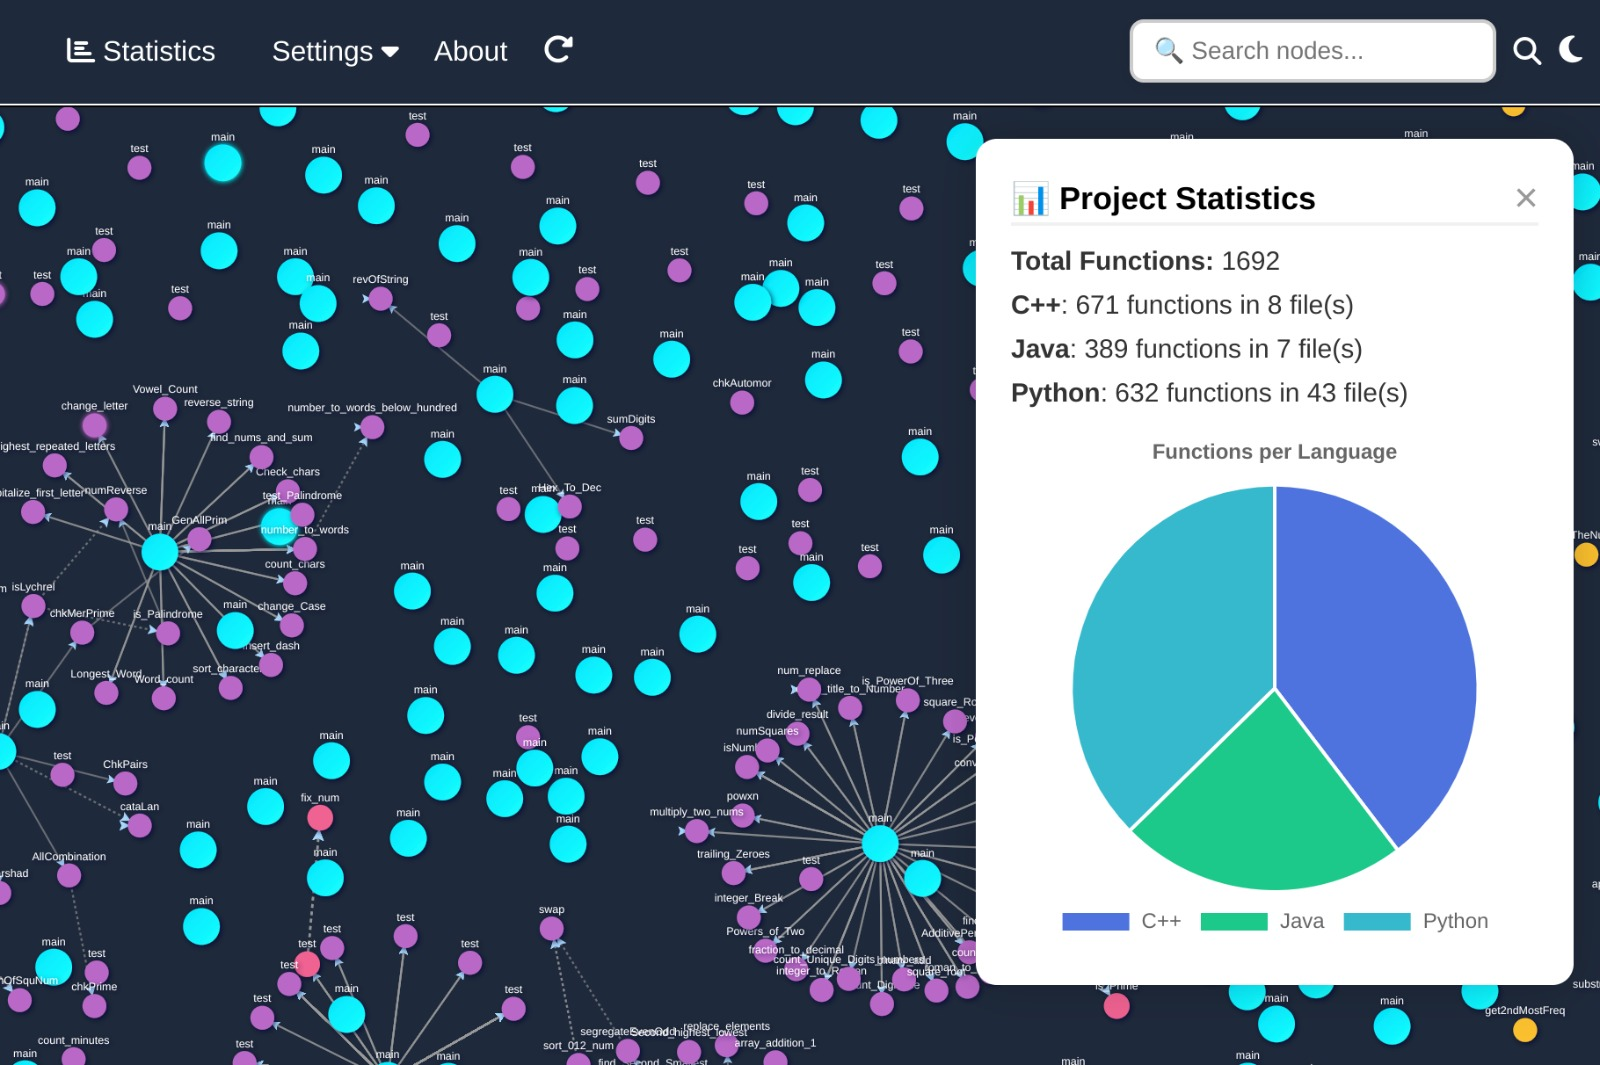
\includegraphics[width=1\linewidth]{Image0.jpg}
    \caption{Folder statistics}
    \label{fig:enter-label}
\end{figure}

\begin{figure}[h]
    \centering
    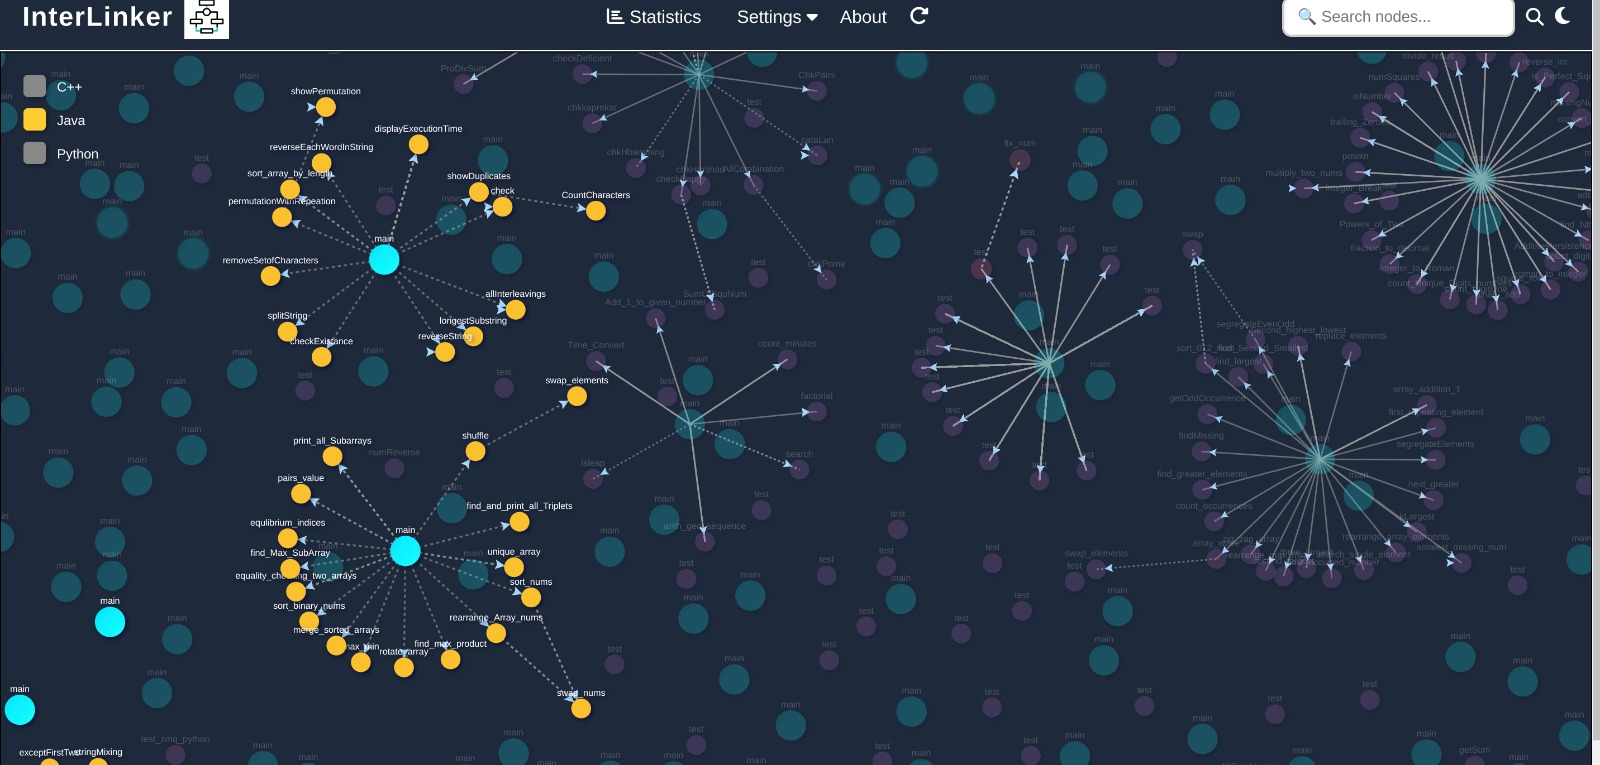
\includegraphics[width=0.45\textwidth]{img1.jpeg}
    \caption{Multi-language Function Graph: Nodes represent functions from different languages}
\end{figure}

\subsection{Visualizing Function Calls Between Languages}

The tool's primary strength is revealing the connections between functions across different languages. Using the D3.js visualization, developers can see a force-directed graph where nodes represent functions and edges represent calls between them. Different colors indicate different programming languages, making cross-language calls immediately apparent.

\begin{figure}[h]
    \centering
    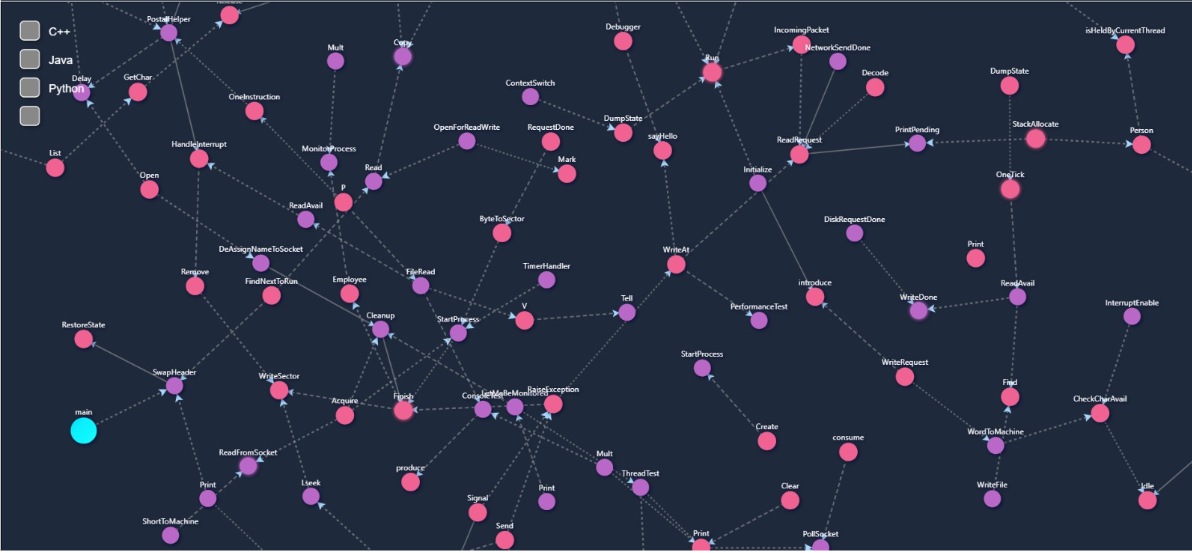
\includegraphics[width=0.45\textwidth]{img2.png}
    \caption{Function Call Visualization: Edges show calls between functions}
\end{figure}

\subsection{Examining Call Context}

A key feature is the ability to see the context in which functions are called. The JSON data structure captures whether calls occur inside conditionals (if/switch statements) or loops, providing insight into control flow. This contextual information is visually encoded in the graph and available in detail views.

\begin{figure}[h]
    \centering
    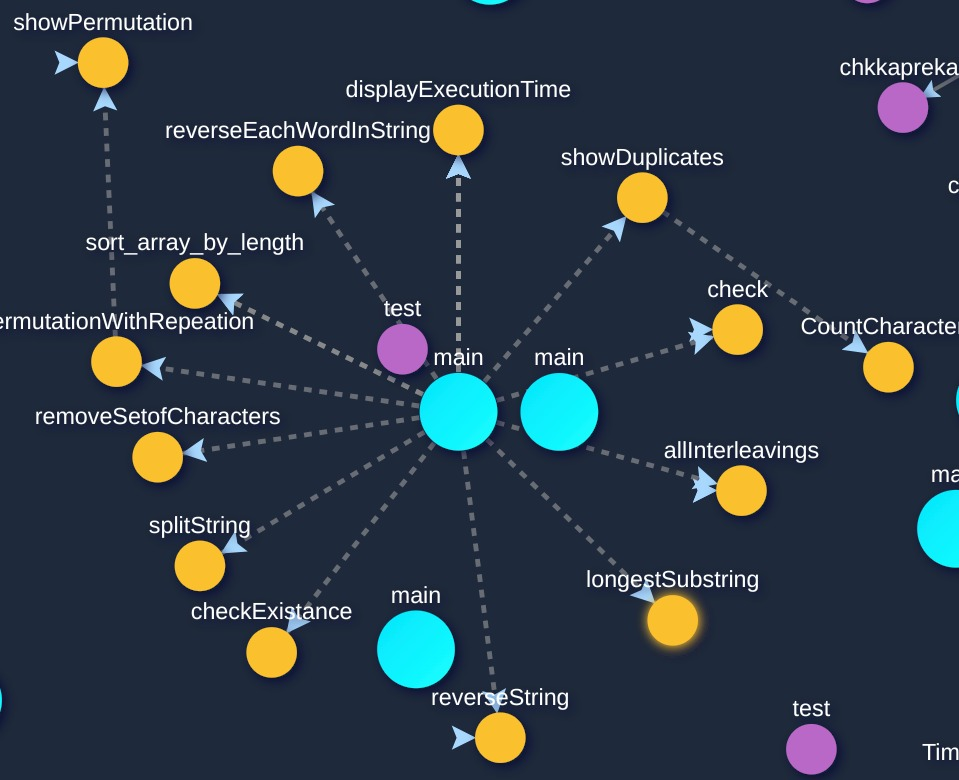
\includegraphics[width=0.45\textwidth]{img3.jpeg}
    \caption{Call Context Visualization: Highlighting functions called within conditionals}
\end{figure}


\subsection{Accessing Function Metadata}

When clicking on a node in the graph, the developer sees detailed metadata about the function, including:
\begin{itemize}
    \item Function name and unique ID
    \item File path and language
    \item Parameter count and types
    \item Parent class and parent function (if nested)
    \item DeepSeek-generated function summary
\end{itemize}

This metadata helps understand the function's purpose without having to open and read the source code directly.

\begin{figure}[h]
    \centering
    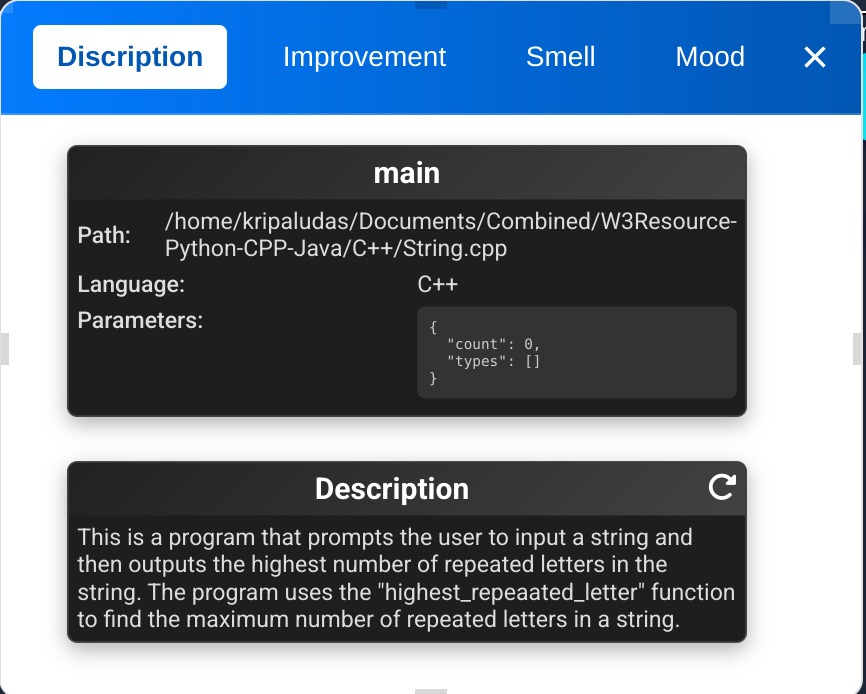
\includegraphics[width=0.45\textwidth]{img4.jpeg}
    \caption{Function Metadata: Detailed information display on node click}
\end{figure}

\subsection{Analyzing Code Using LLM Integration}

The tool leverages DeepSeek to generate concise descriptions of functions, identify code smells, and suggest improvements. These insights are displayed as part of the node metadata, helping developers understand complex functions and identify potential issues for refactoring.

\begin{figure}
    \centering
    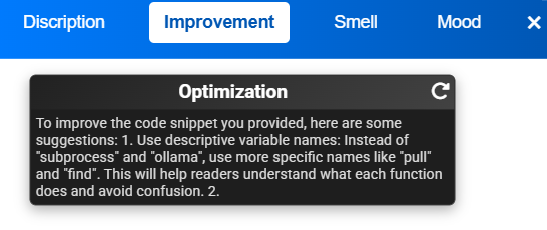
\includegraphics[width=1\linewidth]{img5.png}
    \caption{LLM Analysis: LLM-generated function summaries and improvement suggestions}
    \label{fig:enter-label}
\end{figure}

\begin{figure}
    \centering
    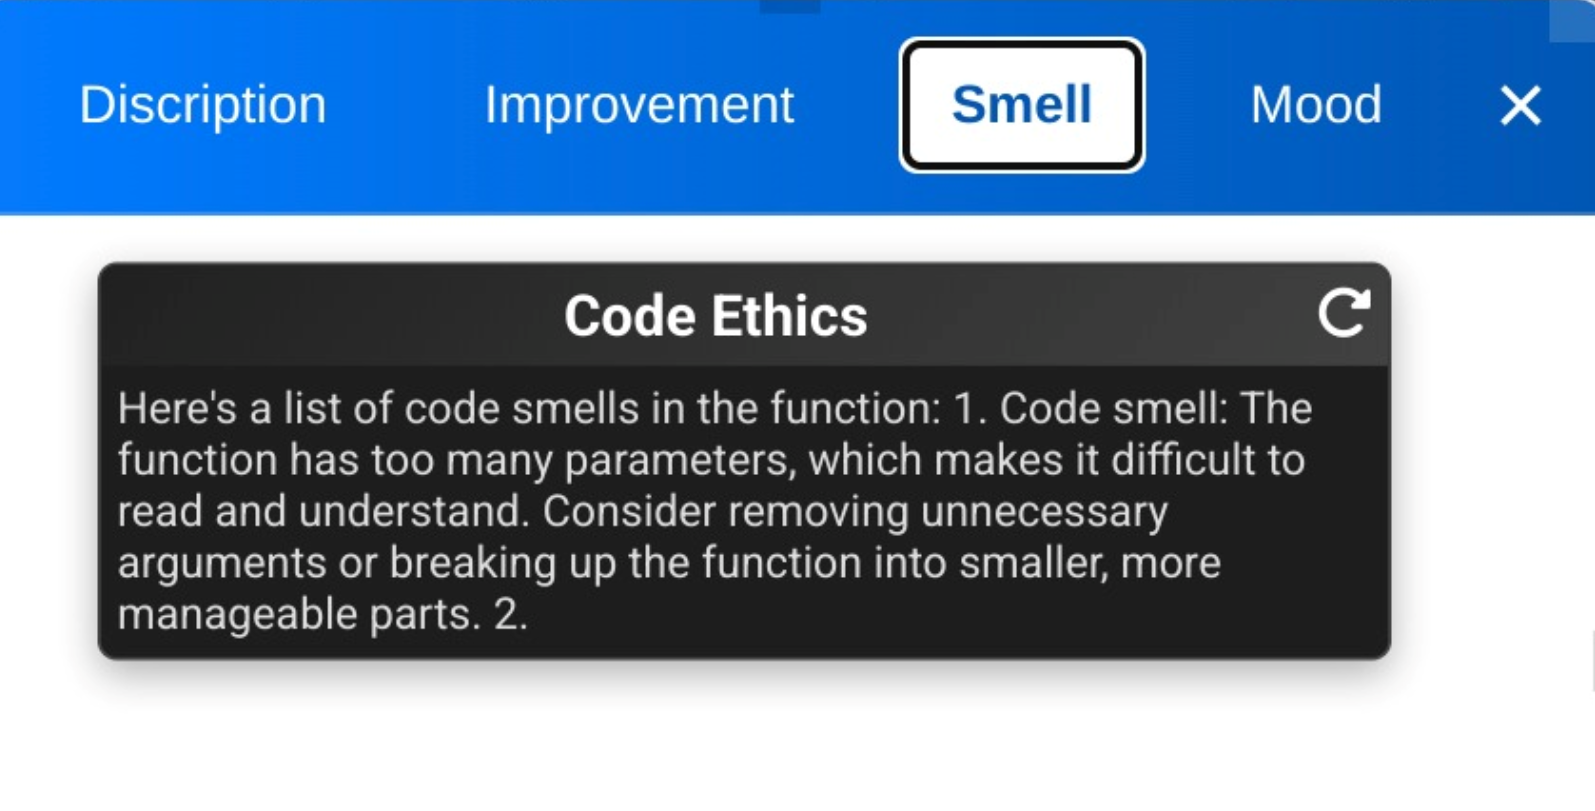
\includegraphics[width=1\linewidth]{image6.png}
    \caption{LLM Analysis: LLM-generated code smell}
    \label{fig:enter-label}
\end{figure}
Through this workflow, our Multi-language Functional Flow Visualization tool makes it significantly easier to understand complex codebases that span multiple programming languages, helping developers navigate unfamiliar code more efficiently.

\section{Discussion \& Limitations}

Our Multi-language Functional Flow Visualization tool aims to simplify understanding of complex, multi-language codebases by providing interactive visual representations of function relationships across language boundaries.

\subsection{Benefits}

The tool provides several advantages:
\begin{itemize}
    \item \textbf{Cross-language visibility:} The tool shows function calls that cross language boundaries between C++, Python, and Java.
    \item \textbf{Context-aware analysis:} By capturing whether calls occur within conditionals, loops, or nested in classes/functions, developers gain deeper insight into execution flow.
    \item \textbf{Standardized JSON format:} The tool outputs a consistent JSON format with uniqueFunctions[] and functionCalls[] arrays, making the data easy to process.
    \item \textbf{DeepSeek integration:} Function summarization and code smell detection provide additional context beyond basic static analysis.
\end{itemize}

\subsection{Limitations}

Despite its utility, our tool also has certain limitations:
\begin{itemize}
    \item \textbf{Limited language support:} Currently only supports Python, Java, and C++.
    \item \textbf{Static analysis constraints:} Dynamic language features may not be fully captured through static analysis.
    \item \textbf{Visualization complexity:} Very large codebases may result in complex graphs that are difficult to navigate.
\end{itemize}

\subsection{Future Work}

As outlined in our Release-2 plan, we aim to address current limitations by:
\begin{itemize}
    \item Improving accuracy of function call detection in current languages
    \item Adding inter-language call detection for Python and Java
    \item Implementing functionality grouping with color-coding for modules
    \item Developing hotspot analysis to identify areas with concentrated function calls
    \item Enhancing refactoring suggestions using AI
    \item Adding metrics and reporting capabilities
\end{itemize}
\section{Discussion and Limitations}

\subsection{Discussion}

The Multi-language Functional Flow Visualization tool offers a powerful means of understanding and navigating large, multi-language codebases, which is especially valuable for developers working in environments that involve complex, cross-language interactions. By extracting and visualizing function definitions and calls, the tool provides a clear view of the functional flow across languages like C++, Python, and Java. This capability enables developers to quickly identify relationships and dependencies between functions, even when they are spread across different files, modules, or languages.

One of the primary strengths of the tool is its ability to visualize cross-language interactions. Traditional tools often focus on single-language projects, but this tool goes a step further by capturing interactions between C++, Python, and Java functions. This feature is particularly useful in modern software systems where different languages are often used for different parts of the system (e.g., C++ for performance-critical components, Python for data processing, and Java for web or enterprise applications).

The interactive visualization of function calls is another key strength. By leveraging D3.js, the tool allows developers to interact with the function graph directly, enabling them to explore the relationships between functions, view function metadata, and identify areas that require further investigation or optimization. This approach is far more intuitive than traditional, static documentation, which can often be difficult to navigate, especially for larger projects.

Additionally, the integration of function summaries and code smell detection through the DeepSeek system provides valuable insights into the code quality. Developers can identify inefficient, redundant, or problematic code that may need to be refactored, improving code maintainability and performance over time.

However, there are areas in which the tool can be improved, especially in terms of scalability and functionality. The next section outlines some of the limitations of the current system.

\subsection{Limitations}

While the Multi-language Functional Flow Visualization tool offers several advantages, there are some inherent limitations that should be addressed in future versions.

\textbf{1. Scalability:}  
As the tool relies on extracting and processing function definitions and calls from potentially large codebases, its performance can degrade as the size and complexity of the project grow. The frontend, built with D3.js, might face performance bottlenecks when rendering large graphs with thousands of nodes and edges. Although optimizations were made to improve rendering performance, there is still room for enhancement to handle larger codebases more efficiently. Techniques like graph partitioning, lazy loading, or virtual rendering could be explored in future iterations.

\textbf{2. Cross-language Call Detection:}  
While the tool currently detects cross-language calls between C++, Python, and Java, its detection mechanism is based on known interop APIs. This approach may miss function calls between languages that are not explicitly defined through interop libraries. Moreover, complex call patterns that involve dynamic function calls or reflection might not be captured effectively, limiting the tool's ability to detect certain cross-language interactions.

\textbf{3. Support for More Languages:}  
Currently, the tool supports only C++, Python, and Java. While these are among the most commonly used languages in multi-language codebases, there are other popular languages (e.g., JavaScript, Ruby, Go) that are not currently supported. Expanding the tool to handle more languages would increase its applicability in diverse development environments. This would require implementing additional parsers and handling language-specific idiosyncrasies.

\textbf{4. Nested Functions and Classes:}  
The tool does well in detecting function calls and class nesting, but there are certain edge cases where deeply nested functions or classes might not be captured accurately. In some cases, the metadata associated with functions, such as their parameters or class context, may not be fully captured due to limitations in the parsing mechanisms. This could lead to incomplete or inaccurate visualizations in more complex code structures.

\textbf{5. Code Smell Detection:}  
The code smell detection feature, powered by DeepSeek, is still in its early stages. While it can identify some obvious issues, such as redundant code or inefficient structures, it is not a comprehensive static code analysis tool. There are many types of code smells (e.g., large functions, deep inheritance hierarchies) that require more sophisticated analysis. Future versions could integrate additional static analysis tools to provide a broader set of code quality insights.

\textbf{6. Docker Environment Setup:}  
While Dockerization ensures that the tool can be run in a consistent environment, setting up Docker for users unfamiliar with containerization could present challenges. Detailed documentation and perhaps even pre-configured Docker images for common development setups could improve the accessibility of the tool.

\section{Future Work}

Several aspects of the tool can be further developed to overcome the limitations discussed. Key areas for future work include:

\begin{itemize}
    \item Enhancing performance for large codebases by exploring advanced graph rendering techniques.
    \item Expanding language support to include other popular programming languages such as Rust, Ruby, and Go.
    \item Improving cross-language call detection, particularly for dynamic or reflection-based function calls.
    \item Integrating more sophisticated code analysis tools to improve code smell detection and provide more actionable insights.
    \item Adding more advanced functionality for identifying hotspots and potential areas for refactoring in large codebases.
\end{itemize}

By addressing these limitations, the tool can become a more robust and scalable solution for visualizing and analyzing multi-language codebases.

\section{Conclusion}

The Multi-language Functional Flow Visualization tool provides valuable insights into large, multi-language codebases by visualizing function calls across languages like C++, Python, and Java. Its interactive visualizations, along with DeepSeek integration for function summaries and code smell detection, enhance developers' ability to understand and navigate complex systems.

While effective, the tool can be improved in scalability, language support, and detection accuracy. Future developments could expand language support, enhance inter-language call detection, and integrate additional code analysis features.

Overall, the tool offers a promising solution for improving code comprehension and software quality in large-scale projects.

\section*{References}
\begin{enumerate}[label={[R\arabic*]}]
    \item D3.js - Data-Driven Documents. \url{https://d3js.org/}
    \item Clang: a C language family frontend for LLVM. \url{https://clang.llvm.org/}
    \item Python Abstract Syntax Tree module. \url{https://docs.python.org/3/library/ast.html}
    \item Javalang: Pure Python library for parsing Java source code. \url{https://github.com/c2nes/javalang}
    \item DeepSeek: AI for Code Analysis. \url{https://www.deepseek.com/}
    \item Docker Documentation. \url{https://docs.docker.com/}
    \item Force-directed Graph Layout Algorithms. \url{https://en.wikipedia.org/wiki/Force-directed_graph_drawing}
    \item Static Code Analysis for Multiple Languages. \url{https://www.perforce.com/blog/sca/what-static-analysis}
\end{enumerate}
\end{document}